% Diagram arsitektur sistem (standalone TikZ) — kompilasi: pdflatex arsitektur_sistem.tex
% Sumber setara dengan arsitektur_sistem.png yang tertanam di makalah.
\documentclass[border=4pt]{standalone}
\usepackage{times}
\usepackage{tikz}
\usetikzlibrary{arrows.meta,positioning,fit,backgrounds}
\begin{document}
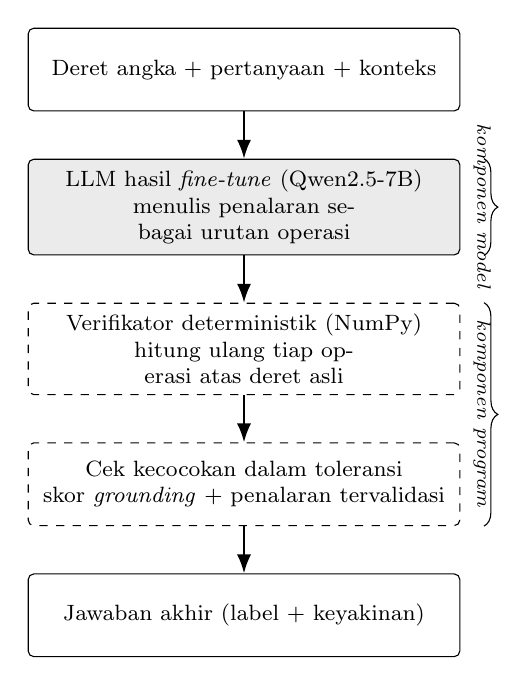
\begin{tikzpicture}[
  font=\footnotesize,
  box/.style={draw,rounded corners=2pt,align=center,text width=5.2cm,
              minimum height=1.05cm,inner sep=4pt},
  prog/.style={box,dashed},
  model/.style={box,fill=black!8},
  arr/.style={-{Latex[length=2.4mm]},thick},
  node distance=6mm and 0mm]
  \node[box]   (in)  {Deret angka + pertanyaan + konteks};
  \node[model] (m)   [below=of in]  {LLM hasil \emph{fine-tune} (Qwen2.5-7B)\\ menulis penalaran sebagai urutan operasi};
  \node[prog]  (v)   [below=of m]   {Verifikator deterministik (NumPy)\\ hitung ulang tiap operasi atas deret asli};
  \node[prog]  (c)   [below=of v]   {Cek kecocokan dalam toleransi\\ skor \emph{grounding} + penalaran tervalidasi};
  \node[box]   (out) [below=of c]   {Jawaban akhir (label + keyakinan)};
  \foreach \a/\b in {in/m,m/v,v/c,c/out} \draw[arr] (\a) -- (\b);
  \draw[decorate,decoration={brace,amplitude=5pt}]
    ([xshift=3mm]m.north east) -- ([xshift=3mm]m.south east)
    node[midway,right=6pt,rotate=-90,anchor=north]{\scriptsize\emph{komponen model}};
  \draw[decorate,decoration={brace,amplitude=5pt}]
    ([xshift=3mm]v.north east) -- ([xshift=3mm]c.south east)
    node[midway,right=6pt,rotate=-90,anchor=north]{\scriptsize\emph{komponen program}};
\end{tikzpicture}
\end{document}
